\newSec[Flight]{Analyse realer Flugdaten}{2}

In diesem Kapitel werden die Daten eines Testflugs mit der \Ar\ analysiert.






\newSec[FlightProcess]{Verlauf}{3}
Dieses Kapitel zeigt die verschiedenen Daten des Flugs, um diese in der nachfolgenden Analyse einordnen zu können.



\begin{figure}[ht!]
\vspace{0.25cm}
\begin{center}
\fbox{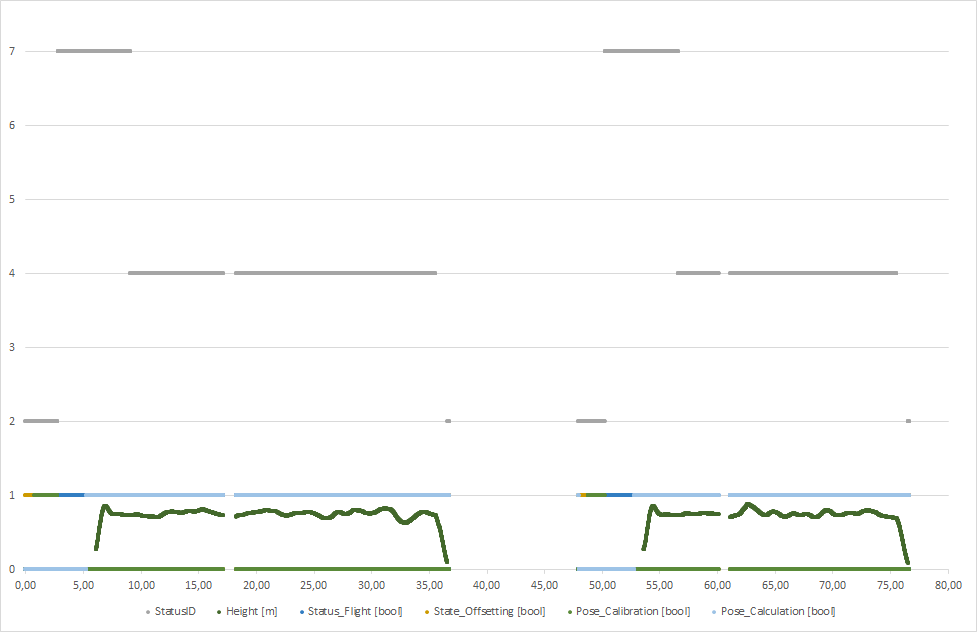
\includegraphics[width=15cm]{Pictures/TestFlight Status Flags Height.png}}
\caption{Testflug: StatusID}
\label{fig:FlightStatus}
\end{center}

\vspace{0.25cm}


\missing[override!!]\\
Der Testflug wird mit der Aufforderung der Status-Änderung bei etwa 9.3 s initialisiert. Davor befindet sich der \Quad\ ruhend auf einer ebenenen Oberfläche.
Die hier eingenommene StatusID = 7 entspricht \glq Goto Fix Point\grq, wobei hier vermutlich eine Höhe von 0.4 m angenommen werden soll. Zwischen etwa 12.3 s und 13.3 s wird keine Nachricht zum aktualisieren der Daten gesendet. Anschließend wechselt der Status zu \grq Flying\glq.
Die Status-Änderung bei etwa 20.6 s entspricht einer Notlandung aufgrund niedriger Batterieladung.
\end{figure}


\begin{figure}[ht!]
\vspace{0.25cm}
\begin{center}
\fbox{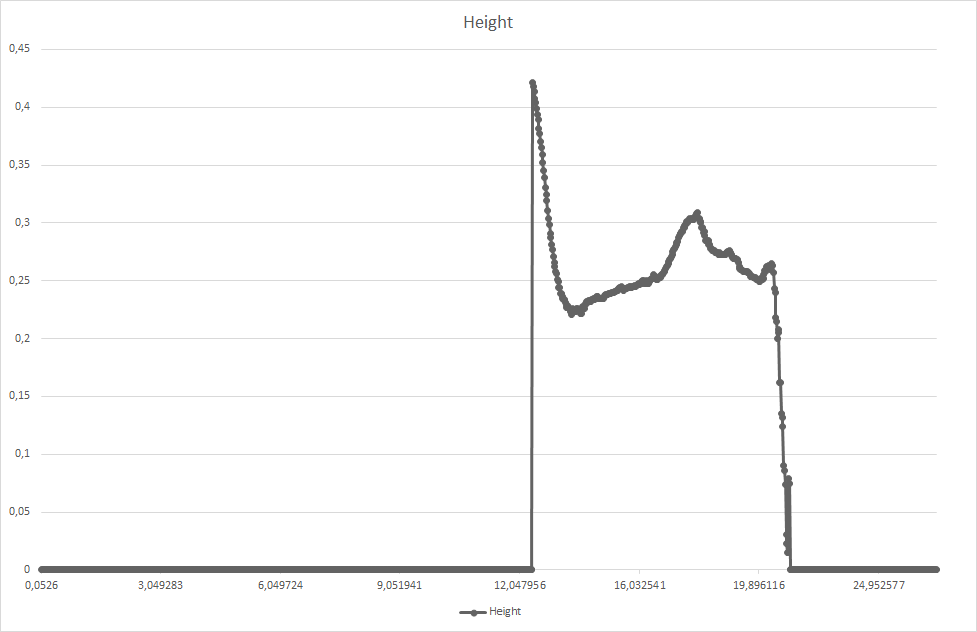
\includegraphics[width=15cm]{Pictures/Flight Height.png}}
\caption{Testflug: Höhenverlauf}
\label{fig:FlightHeight}
\end{center}

\vspace{0.25cm}
Äquivalent zu \refImg{fig:FlightStatus} zeigt sich der Verlauf des Höhenprofils des Fluges. Die Daten wurden von der Ultraschall-Messung abgegriffen. Eine Transformation der Einheiten in [$m$] wurde vorgenommen.
\end{figure}









\missing[Analyse mit Daten der parrot Drohne]









\FloatBarrier
\newSec[FlightAnalysis]{Analyse}{3}


\newSec[FlightAnalysisLeak]{Lecks der Datenübertragung}{4}

\missing[Beim Start etwa 1s, etwas später nochmal ein bisschen Probleme...]





\newSec[FlightAnalysisOffset]{Offset der Beschleunigungswerte}{4}

Wie \refImg{fig:Flightaxay} entnommen werden kann, sind die Werte für die Bescleunigungen entlang der x- und y-Achsen nicht auf den Wert 0 kalibriert. Eine Kalibrierung des \Quad[s] wird unmittelbar vor dem Start gesendet und kann auch unabhängig durch eine User-Eingabe ausgelöst werden.

Die Gravitation ist in \refImg{fig:Flightaz} ablesbar.

Entsprechend \refCap{ControlPosAccelOffset} sind diese Abweichungen zu korrigieren.
Als Ansatz kann hier eine Mittlung der Werte bis zum Senden der Start-Aufforderung gewählt werden. Aus \refImg{fig:Flightaxay} und \refImg{fig:Flightaz} ist ersichtlich, dass hier keine signifikanten Schwankungen auftreten. 





\newSec[FlightAnalysisReconstruction]{Rekonstruktion der Flughöhe}{4}






Bei beiden Filtern ist eine deutliche Abweichung ersichtlich.

\missing[was ist hier los?]
entsprechend \refCap{ControlPosAccelOffset} um

Aus der Rekonstruktion in \refImg{fig:FlightHeightReconst} lässt sich zeigen, dass markante Verläufe abgebildet werden können.

Die rekonstruierte Kurve ist jedoch in den negativen Bereich verschoben. Dies lässt sich mit der fehlenden Datenübertragung beim Start des \Quad[s] begründen. 
Darüber hinaus ist eine konstante Geschwindigkeit nach der Landung anhand der konstanten Steigung der rekonstruierten Kurve in diesem Bereich ersichtlich.









